%%%%%%%%%%%%%%%%%%%%%%%%%%%%%%%%%%%%%%%%%
% Beamer Presentation
% LaTeX Template
% Version 1.0 (10/11/12)
%
% This template has been downloaded from:
% http://www.LaTeXTemplates.com
%
% License:
% CC BY-NC-SA 3.0 (http://creativecommons.org/licenses/by-nc-sa/3.0/)
%
%%%%%%%%%%%%%%%%%%%%%%%%%%%%%%%%%%%%%%%%%

%----------------------------------------------------------------------------------------
%	PACKAGES AND THEMES
%----------------------------------------------------------------------------------------

\documentclass[UTF8,aspectratio=169,14pt]{ctexbeamer}

\usepackage{hyperref}
\hypersetup{
	colorlinks=true,
	linkcolor=red,
	anchorcolor=blue,
	citecolor=green
}

\mode<presentation> {
	
	% The Beamer class comes with a number of default slide themes
	% which change the colors and layouts of slides. Below this is a list
	% of all the themes, uncomment each in turn to see what they look like.
	
	%\usetheme{default}
	%\usetheme{AnnArbor}
	%\usetheme{Antibes}
	%\usetheme{Bergen}
	%\usetheme{Berkeley}
	%\usetheme{Berlin}
	%\usetheme{Boadilla}
	%\usetheme{CambridgeUS}
	%\usetheme{Copenhagen}
	%\usetheme{Darmstadt}
	%\usetheme{Dresden}
	%\usetheme{Frankfurt}
	%\usetheme{Goettingen}
	%\usetheme{Hannover}
	%\usetheme{Ilmenau}
	%\usetheme{JuanLesPins}
	%\usetheme{Luebeck}
	\usetheme{Madrid}
	%\usetheme{Malmoe}
	%\usetheme{Marburg}
	%\usetheme{Montpellier}
	%\usetheme{PaloAlto}
	%\usetheme{Pittsburgh}
	%\usetheme{Rochester}
	%\usetheme{Singapore}
	%\usetheme{Szeged}
	%\usetheme{Warsaw}
	
	% As well as themes, the Beamer class has a number of color themes
	% for any slide theme. Uncomment each of these in turn to see how it
	% changes the colors of your current slide theme.
	
	%\usecolortheme{albatross}
	%\usecolortheme{beaver}
	%\usecolortheme{beetle}
	%\usecolortheme{crane}
	%\usecolortheme{dolphin}
	%\usecolortheme{dove}
	%\usecolortheme{fly}
	%\usecolortheme{lily}
	%\usecolortheme{orchid}
	%\usecolortheme{rose}
	%\usecolortheme{seagull}
	%\usecolortheme{seahorse}
	%\usecolortheme{whale}
	%\usecolortheme{wolverine}
	
	%\setbeamertemplate{footline} % To remove the footer line in all slides uncomment this line
	%\setbeamertemplate{footline}[page number] % To replace the footer line in all slides with a simple slide count uncomment this line
	
	%\setbeamertemplate{navigation symbols}{} % To remove the navigation symbols from the bottom of all slides uncomment this line
}

\usepackage{graphicx} % Allows including images
\graphicspath{{./figs/}}
\usepackage{booktabs} % Allows the use of \toprule, \midrule and \bottomrule in tables
\usepackage{longtable}
\usepackage{listings}
\usepackage{xcolor}
\lstset{numbers=left, %设置行号位置
	numberstyle=\tiny, %设置行号大小
	keywordstyle=\color{blue}, %设置关键字颜色
	commentstyle=\color[cmyk]{1,0,1,0}, %设置注释颜色
	frame=single, %设置边框格式
	escapeinside=``, %逃逸字符(1左面的键),用于显示中文
	%breaklines, %自动折行
	extendedchars=false, %解决代码跨页时,章节标题,页眉等汉字不显示的问题
	xleftmargin=2em,xrightmargin=2em, aboveskip=1em, %设置边距
	tabsize=4, %设置tab空格数
	showspaces=false %不显示空格
}
% Fonts
% \usepackage{libertine}
% \setmonofont{Courier}
\setCJKsansfont[ItalicFont=Noto Serif CJK SC Black, BoldFont=Noto Sans CJK SC Black]{Noto Sans CJK SC}


%----------------------------------------------------------------------------------------
% TITLE PAGE
%----------------------------------------------------------------------------------------

\title[第21讲]{第二十一讲 :异步编程(Asynchronous Programming)} % The short title appears at the bottom of every slide, the full title is only on the title page
\subtitle{第2节:Futures in Rust}
\author{向勇、陈渝} % Your name
\institute[清华大学] % Your institution as it will appear on the bottom of every slide, may be shorthand to save space
{
  清华大学计算机系 \\ % Your institution for the title page
  \medskip
  \textit{xyong,yuchen@tsinghua.edu.cn} % Your email address
}
\date{\today} % Date, can be changed to a custom date

\begin{document}

\begin{frame}
\titlepage % Print the title page as the first slide
\end{frame}

%----------------------------------------------
\begin{frame}
\frametitle{提纲} % Table of contents slide, comment this block out to remove it
\tableofcontents % Throughout your presentation, if you choose to use \section{} and \subsection{} commands, these will automatically be printed on this slide as an overview of your presentation

%% itemize
Ref:
    \begin{itemize}
        \item \href{}{xxxx}
    \end{itemize}

\end{frame}
%----------------------------------------------
%%  PRESENTATION SLIDES
%----------------------------------------------
\section{第2节:Futures in Rust} % Sections can be created in order to organize your presentation into discrete blocks, all sections and subsections are automatically printed in the table of contents as an overview of the talk
%----------------------------------------------
% ### 21.2 Futures in Rust
% 
% 参考: https://cfsamson.github.io/books-futures-explained/1_futures_in_rust.html#futures-in-rust
% 参考: https://github.com/cfsamson/books-futures-explained
% 参考: Evernote: 20200402-异步消息调研
% 
%----------------------------------------------
\begin{frame}[fragile]
    \frametitle{零成本异步I/O}
%    \framesubtitle{xxxx}
% #### 零成本异步I/O
% 
% 参考:
% 
% - video https://www.youtube.com/watch?v=skos4B5x7qE
% - 中文 https://zhuanlan.zhihu.com/p/97574385
% - async汇总 https://areweasyncyet.rs/
% 
Future的设计目标

%% itemize
    \begin{itemize}
        \item 调用 I/O 时,系统调用会立即返回,然后你可以继续进行其他工作
        \item I/O完成时,回到调用该异步 I/O 暂停的那个任务线上
        \item {\color{red}一种通过对异步 I/O 的良好抽象形成的基于库的解决方案}
    	\begin{itemize}
    	    \item 它不是语言的一部分,也不是每个程序附带的运行时的一部分,只是可选的并按需使用的库
    	\end{itemize}
    \end{itemize}

{\color{red}零成本抽象}
% 
%% itemize
    \begin{itemize}
        \item 不给不使用该功能的用户增加成本
        \item 使用该功能时,它的速度不会比不使用它的速度慢
    \end{itemize}
% 
\end{frame}
%----------------------------------------------
\begin{frame}[fragile]
    \frametitle{Concept of Future}
%    \framesubtitle{xxxx}
% #### Concept of Future
% 
% Ref: https://os.phil-opp.com/async-await/#example
% 
A future is a representation of some operation which will complete in the future.
% 
%% figure
    \begin{figure}
    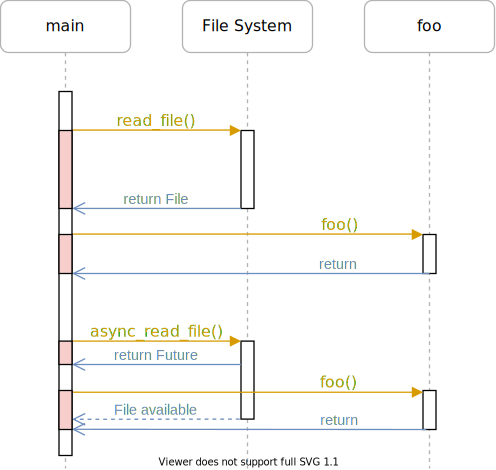
\includegraphics[width=0.8\linewidth]{figs/async-example.svg}
%    \caption{xxxx}
    \end{figure}
% ![async-example](figs/async-example.svg)
% 
Three phases in asynchronous task:
% 
    \begin{itemize}
        \item {\color{red}Executor}: A Future is polled which result in the task progressing
    	\begin{itemize}
    	    \item Until a point where it can no longer make progress
    	\end{itemize}
        \item {\color{red}Reactor}: Register an event source that a Future is waiting for
    	\begin{itemize}
    	    \item Makes sure that it will wake the Future when that event is ready
    	\end{itemize}
        \item {\color{red}Waker}: The event happens and the Future is woken up
    	\begin{itemize}
    	    \item Wake up to the executor which polled the Future
    	    \item Schedule the future to be polled again and make further progress
    	\end{itemize}
    \end{itemize}
% 
\end{frame}
%----------------------------------------------
\begin{frame}[fragile]
    \frametitle{基于轮询的 Future的异步执行过程}
%    \framesubtitle{xxxx}
% #### 基于轮询的 Future的异步执行过程
% 
%% itemize
    \begin{itemize}
        \item 执行器会轮询 `Future`,直到最终 `Future` 需要执行某种 I/O 
        \item 该 `Future` 将被移交给处理 I/O 的反应器,即 `Future` 会等待该特定 I/O 
        \item I/O 事件发生时,反应器将使用传递的`Waker` 参数唤醒 `Future` ,传回执行器
        \item 循环上述三步,直到最终`future`任务完成(resolved)
        \item 任务完成并得出结果时,执行器释放句柄和整个`Future`,整个调用过程就完成了
    \end{itemize}
% 
%% figure
    \begin{figure}
    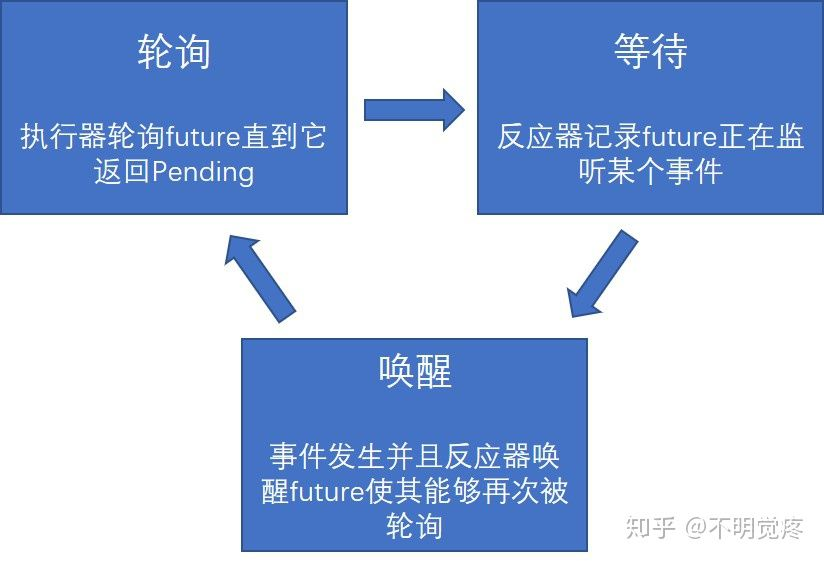
\includegraphics[width=0.8\linewidth]{figs/future-loop.jpg}
%    \caption{xxxx}
    \end{figure}
% ![future-loop](figs/future-loop.jpg)
% 
\end{frame}
%----------------------------------------------
\begin{frame}[fragile]
    \frametitle{Leaf futures \& Non-leaf-futures}
%    \framesubtitle{xxxx}
% #### Leaf futures & Non-leaf-futures
% 
% Ref: https://cfsamson.github.io/books-futures-explained/1_futures_in_rust.html#leaf-futures
% 
% Ref: https://os.phil-opp.com/async-await/#the-async-await-pattern
% 
    \begin{itemize}
        \item Leaf future
    	\begin{itemize}
    	    \item Runtimes create *leaf futures* which represents a resource like a socket
    	    \item Operations on these resources will be non-blocking and return a future which we call a leaf future
    	\end{itemize}
% ```rust
% // stream is a {\color{red}leaf-future}
% let mut stream = tokio::net::TcpStream::connect("127.0.0.1:3000");
% ```

        \item Non-leaf-future
    	\begin{itemize}
    	    \item The bulk of an async program will consist of non-leaf-futures, which are a kind of pause-able computation
    	    \item Non-leaf-futures represents a *set of operations*
    	\end{itemize}
    \end{itemize}
% 
% ```rust
% // Non-leaf-future
% async fn example(min_len: usize) -> String {
%     let content = async_read_file("foo.txt").await;
%     if content.len() < min_len {
%         content + &async_read_file("bar.txt").await
%     } else {
%         content
%     }
% }
% ```
% 
\end{frame}
%----------------------------------------------
\begin{frame}[fragile]
    \frametitle{Runtimes}
%    \framesubtitle{xxxx}
% #### Runtimes
%% itemize
    \begin{itemize}
        \item Languages like C\#, JavaScript, Java, GO and many others comes with a runtime for handling concurrency
        \item Rust uses a library for handling concurrency

        \item The two most popular runtimes for Futures:
    	\begin{itemize}
    	    \item \href{https://github.com/async-rs/async-std}{async-std}
    	    \item \href{https://github.com/tokio-rs/tokio}{Tokio}
    	\end{itemize}
    \end{itemize}
% 
{\color{red}What Rust's standard library takes care of}
% ref: https://cfsamson.github.io/books-futures-explained/1_futures_in_rust.html#what-rusts-standard-library-takes-care-of
% 
    \begin{itemize}
        \item A {\color{red}common interface} representing an operation which will be completed in the future through the `Future` trait.
        \item An ergonomic way of {\color{red}creating tasks} which can be suspended and resumed through the `async` and `await` keywords.
        \item A defined interface wake up a suspended task through the `Waker` type.
    \end{itemize}
% 
\end{frame}
%----------------------------------------------
\begin{frame}[fragile]
    \frametitle{Rust future example}
%    \framesubtitle{xxxx}
% #### Rust future example
% 
% Ref: https://os.phil-opp.com/async-await/#the-async-await-pattern
% 
% ```rust
% use futures::future::{self, Future};
% 
% fn main() {
%     let _ = example(100);
% }
% 
% async fn example(min_len: usize) -> String {
%     let content = async_read_file("foo.txt").await;
%     if content.len() < min_len {
%         content + &async_read_file("bar.txt").await
%     } else {
%         content
%     }
% }
% 
% fn async_read_file(name: &str) -> impl Future<Output = String> {
%     future::ready(String::from(name))
% }
% ```
% 
\end{frame}
%----------------------------------------------
\begin{frame}[fragile]
    \frametitle{Async Lifetimes}
%    \framesubtitle{xxxx}
% #### Async Lifetimes
% 
% Ref: https://rust-lang.github.io/async-book/03_async_await/01_chapter.html#async-lifetimes
% 
%% itemize
    \begin{itemize}
        \item `async fn`s which take references or other non-`'static` arguments return a `Future` which is bounded by the lifetime of the arguments.
    \end{itemize}
% 
% ```rust
% // This function:
% async fn foo(x: &u8) -> u8 { *x }
% 
% // Is equivalent to this function:
% fn foo_expanded<'a>(x: &'a u8) -> impl Future<Output = u8> + 'a {
%     async move { *x }
% }
% ```
% 
%% itemize
    \begin{itemize}
        \item By moving the argument into the `async` block, we extend its lifetime to match that of the `Future` returned
    \end{itemize}
% 
% ```rust
% fn bad() -> impl Future<Output = u8> {
%     let x = 5;
%     borrow_x(&x) // ERROR: `x` does not live long enough
% }
% 
% fn good() -> impl Future<Output = u8> {
%     async {
%         let x = 5;
%         borrow_x(&x).await
%     }
% }
% ```
% 
\end{frame}
%----------------------------------------------
\begin{frame}[fragile]
    \frametitle{Zero-cost futures in Rust}
%    \framesubtitle{xxxx}
% #### Zero-cost futures in Rust
% 
% Ref: https://aturon.github.io/blog/2016/08/11/futures/
% 
%% itemize
    \begin{itemize}
        \item Build up a big `enum` that represents the state machine
    	\begin{itemize}
    	    \item There is one allocation needed per “task”, which usually works out to one per connection
    	\end{itemize}
        \item When an event arrives, only one dynamic dispatch is required
        \item There are essentially no imposed synchronization costs
    \end{itemize}
% 
Here are the results, in number of “Hello world!"s served per second on an 8 core Linux machine.
% 
%% figure
    \begin{figure}
    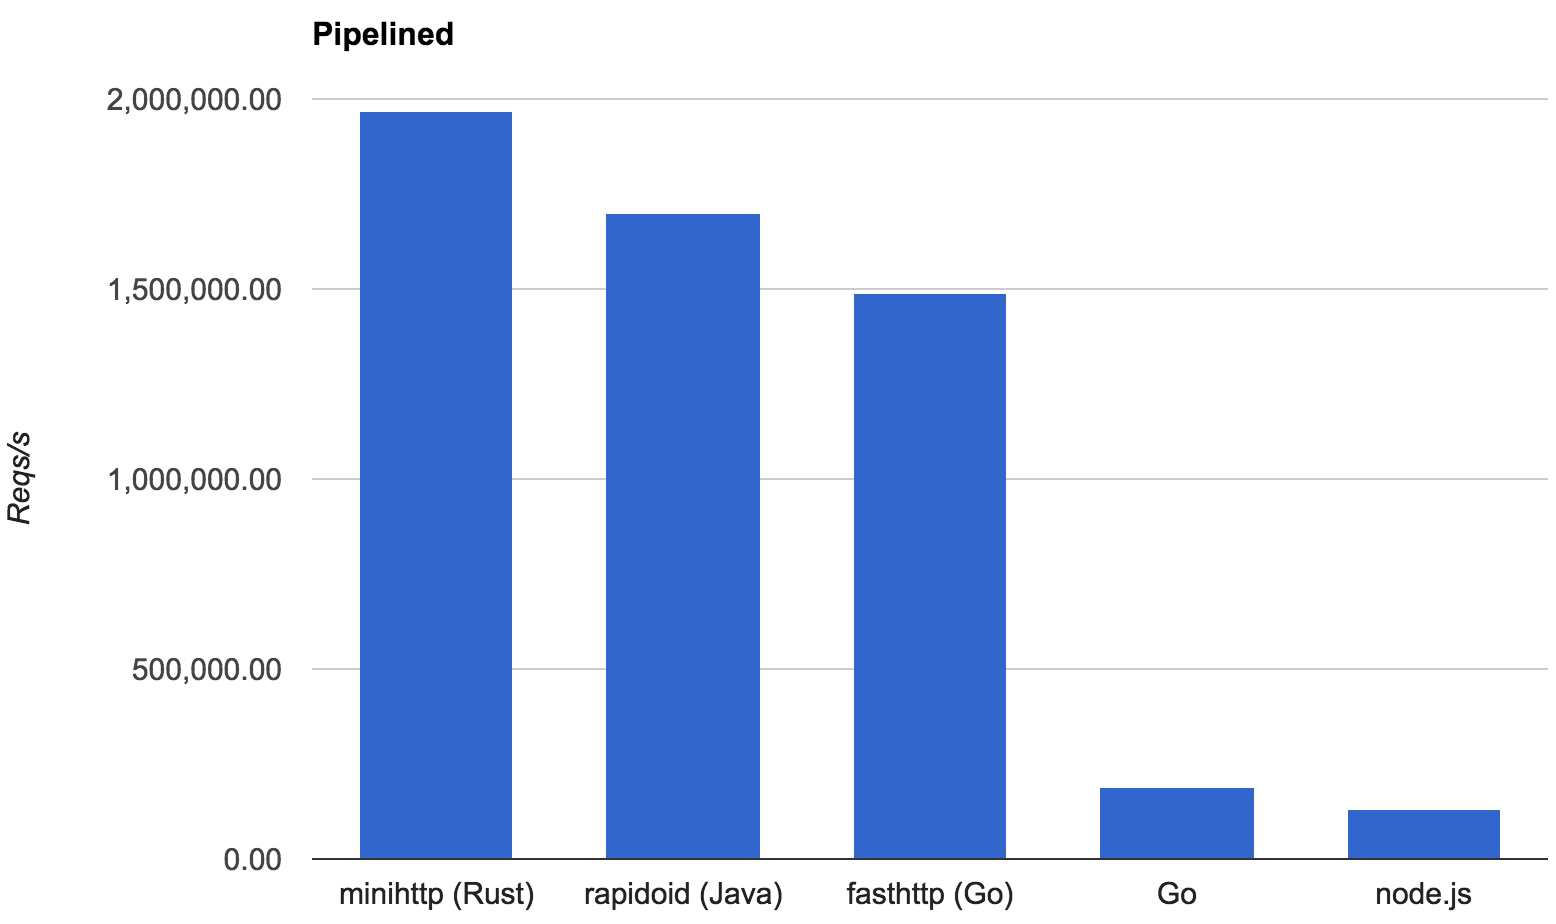
\includegraphics[width=0.8\linewidth]{figs/bench-pipelined.png}
%    \caption{xxxx}
    \end{figure}
% ![bench-pipelined](figs/bench-pipelined.png)
% 
\end{frame}
%----------------------------------------------
\end{document}
